% example.tex
%
% Copyright (C) 2010,2011 Laura Dietz
% Copyright (C) 2012 Jaakko Luttinen
%
% The MIT License
%
% See LICENSE file for more details.

\documentclass[a4paper]{article}

\usepackage{tikz}
\usetikzlibrary{bayesnet}
%\pgfrealjobname{example} % name of this file

\title{Graphical Models in Tikz}
\author{Laura Dietz, Jaakko Luttinen}

\begin{document}

\maketitle

TikZ examples for graphical models (Bayesian networks) and directed
factor graphs \cite{Dietz:2010}.

% A table of node types
\begin{table}[ht]
  \caption{Node types}
  \begin{center}
    \begin{tabular}{llc}
      Type & Syntax & Output
      \\
      \hline
      Latent variable &
      \texttt{\textbackslash node[latent]} &
      \tikz{ %
        \node[latent] {$x$}; %
      }
      \\
      Observed variable &
      \texttt{\textbackslash node[obs]} &
      \tikz{ %
        \node[obs] {$y$}; %
      }
      \\
      Deterministic &
      \texttt{\textbackslash node[det]} &
      \tikz{ %
        \node[det] {dot} ; %
      }
      \\
      Constant &
      \texttt{\textbackslash node[const]} &
      \tikz{ %
        \node[const] {$a$}; %
      }
      \\
      Factor &
      \texttt{\textbackslash node[factor]} &
      \tikz{ %
        \node[factor] [label=$\mathcal{N}$] {}; %
      }
    \end{tabular}
  \end{center}
\end{table}
\begin{table}[ht]
  \caption{Edge types}
  \begin{center}
    \begin{tabular}{llc}
      Type & Syntax & Output
      \\
      \hline
      Directed edges &
      \texttt{\textbackslash edge[opts]\{inputs\}\{outputs\}} &
      \tikz{ %
        \node[obs] (y) {$y$} ; %
        \node[latent, left=of y, yshift=0.5cm] (mu) {$\mu$} ; %
        \node[latent, left=of y, yshift=-0.5cm] (tau) {$\tau$} ; %
        \edge {mu,tau} {y} ; %
      }
      \\
      Undirected edges &
      \texttt{\textbackslash edge[-,opts]\{inputs\}\{outputs\}} &
      \tikz{ %
        \node[obs] (y) {$y$} ; %
        \node[latent, left=of y, yshift=0.5cm] (mu) {$\mu$} ; %
        \node[latent, left=of y, yshift=-0.5cm] (tau) {$\tau$} ; %
        \edge[-] {mu,tau} {y} ; %
      }
      \\
      Factor graph edges &
      \texttt{\textbackslash factoredge[opts]\{inputs\}\{via\}\{outputs\}} &
      \tikz{ %
        \node[obs] (y) {$y$} ; %
        \node[latent, left=of y, yshift=0.5cm] (mu) {$\mu$} ; %
        \node[latent, left=of y, yshift=-0.5cm] (tau) {$\tau$} ; %
        \factor[left=of y] {y-factor} {$\mathcal{N}$} {} {};
        \factoredge {mu,tau} {y-factor} {y} ; %
      }
    \end{tabular}
  \end{center}
\end{table}
\begin{table}[ht]
  \caption{Utilities}
  \begin{center}
    \begin{tabular}{llc}
      Type & Syntax & Output
      \\
      \hline
      Plate &
      \texttt{\textbackslash plate} &
      \tikz{ %
        \node[latent] (x) {$x_m$}; %
        \plate {} {(x)} {$m \in \mathcal{M}$}; %
      }
      \\
      Gate &
      &
      \tikz{
        % Nodes
        \node[obs]                    (k)   {$k$}; %
        \node[latent, above=2 of k]   (l)   {$\lambda$}; %
        \factor[above=0.8 of k]       {k-f} {Multi} {} {}; %
        \node[latent, right=of k-f]   (paa) {$\phi$}; %
        %\node[latent, right=of k-f]   (p)   {$\phi$}; %
        % Connections
        \factoredge {paa} {k-f} {k} ; %
        % Gate
        \gate {} {(k-f)(k-f-caption)} {l} ; %
      }
    \end{tabular}
  \end{center}
\end{table}


% Simple Bayesian network
\begin{figure}[ht]
  \begin{center}
    \begin{tabular}{cc}
      %\beginpgfgraphicnamed{model-pca}
\begin{tikzpicture}

% Define nodes
\node[obs, xshift = -2cm]   (y2){$y$};
\node[obs, xshift = 0cm] (y1){$y$};
\node[det, above= of {y1, y2}, xshift = -1cm ]     (if) {if-else} ; % 
\node[latent, above= of if]             (x){$x_{n}$};
%\node[latent, above= of y, xshift=0cm]   (true) {$z_{n}$};
%\node[latent, above=of z, xshift=0cm]   (false) {$s$};
%\node[latent, above=of z, xshift=1.2cm]  (b) {$b$};
%\node[obs, above= of z, xshift=-1.2cm]   (x) {$x_{n}$}; 

% Connect the nodes
\edge {x}{if};
\edge [dashed]{if}{y1,y2};

% Plates
%\plate {yx} {(x)(y)} {$N$} ;
%\plate {} {(w)(y)(yx.north west)(yx.south west)} {$M$} ;

\end{tikzpicture}
    \end{tabular}
  \end{center}
  \caption{PCA model as a Bayesian network and a directed factor
    graph.}
\end{figure}

% Latent Dirichlet allocation
\begin{figure}[ht]
  \begin{center}
    % model_pca.tex
%
% Copyright (C) 2012 Jaakko Luttinen
%
% The MIT License
%
% See LICENSE file for more details.

% PCA model

%\beginpgfgraphicnamed{model-pca}
%\begin{tikzpicture}
%
%  % Define nodes
%  \node[obs]                               (y) {$y$};
%  \node[latent, above=of y, xshift=-1.2cm] (w) {$\mathbf{w}$};
%  \node[latent, above=of y, xshift=1.2cm]  (x) {$\mathbf{x}$};
%  \node[latent, right=2cm of y]            (t) {$\tau$};
%
%  % Connect the nodes
%  \edge {x,w,t} {y} ; %
%
%  % Plates
%  \plate {yx} {(x)(y)} {$N$} ;
%  \plate {} {(w)(y)(yx.north west)(yx.south west)} {$M$} ;
%
%\end{tikzpicture}
%\endpgfgraphicnamed

%%% Local Variables: 
%%% mode: tex-pdf
%%% TeX-master: "example"
%%% End: % model_pca.tex
%
% Copyright (C) 2012 Jaakko Luttinen
%
% The MIT License
%
% See LICENSE file for more details.

% PCA model

%\beginpgfgraphicnamed{model-pca}
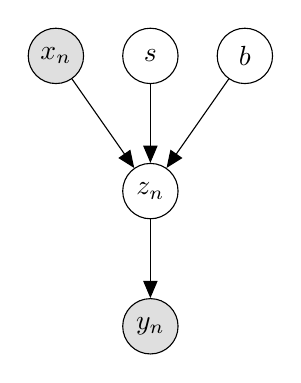
\begin{tikzpicture}

\node[obs](y){$y_{n}$};
% Define nodes
\node[latent, above= of y, xshift=0cm]   (z) {$z_{n}$};
\node[latent, above=of z, xshift=0cm]   (s) {$s$};
\node[latent, above=of z, xshift=1.2cm]  (b) {$b$};
\node[obs, above= of z, xshift=-1.2cm]   (x) {$x_{n}$}; 

% Connect the nodes
\edge {x,s,b} {z} ; %
\edge {z} {y} ;s

% Plates
%\plate {yx} {(x)(y)} {$N$} ;
%\plate {} {(w)(y)(yx.north west)(yx.south west)} {$M$} ;

\end{tikzpicture}
%\endpgfgraphicnamed

%%% Local Variables: 
%%% mode: tex-pdf
%%% TeX-master: "example"
%%% End: 
  \end{center}
  \caption{Latent Dirichlet allocation as directed factor graph.}
\end{figure}

% Citation influence model
%\begin{figure}[ht]
%  \begin{center}
%    \input{model_citation_influence}
%  \end{center}
%  \caption{Citation influence model with own topics \cite{Dietz:2007}
%    as directed factor graph.}
%\end{figure}

\clearpage

\begin{thebibliography}{9}

\bibitem{Dietz:2010}
  Laura Dietz,
  \emph{Directed Factor Graph Notation for Generative Models}.
  Technical Report. 2010

% Laura Dietz, Steffen Bickel, Tobias Scheffer. 
% Unsupervised Prediction of Citation Influences. 
% In: Proceedings of International Conference on Machine Learning. 2007
\bibitem{Dietz:2007}
  Laura Dietz, Steffen Bickel, Tobias Scheffer,
  \emph{Unsupervised Prediction of Citation Influences}.
  In: Proceedings of International Conference on Machine
  Learning. 2007


\end{thebibliography}

\end{document}

%%% Local Variables: 
%%% mode: tex-pdf
%%% TeX-master: t
%%% End: 